
\chapter{基于粒子群算法的软件补偿方法及算法硬化}
\section{粒子群算法}
\subsection{粒子群算法基本原理}

粒子群算法(Particle Swarm optimization,PSO)是一种启发于鸟群协同捕食行为的智能算法,利用种群与个体之间的信息交互来寻找问题的最优解,具有较高的搜索效率和精度\cite{潘红丽2022基于改进粒子群算法的垃圾清运车辆低碳路径规划},已广泛应用于函数优化等领域\cite{2022Environmental}。

\begin{figure}[htb]
  \centering
  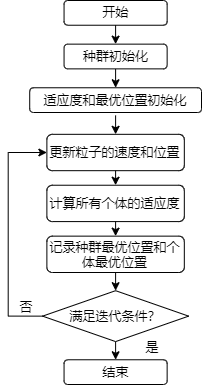
\includegraphics[width=4cm,height=7cm]{fig/4-fig/粒子群算法流程图.png}
  \caption{粒子群算法流程图}
  \label{fig:粒子群算法流程图}
\end{figure}
可以假设这样一个场景:一群鸟在随机的搜寻食物,并且搜寻空间里只有一块食物,所有的鸟都不知道食物在哪里,并且所有鸟的初始位置和搜寻方向都是随机的。在该场景下,一个找寻食物的最优策略就是搜寻离食物最近的鸟的周围。距离食物的距离就代表着优化效果的好坏,而鸟群每个时刻所处在的位置,就代表着粒子群算法覆盖到的迭代值,整个空间即为粒子群算法的搜索空间,将该方式抽象成算法,如图\ref{fig:粒子群算法流程图}所示。

由图\ref{fig:粒子群算法流程图}中可以看出,粒子群算法的第一步是对种群进行初始化,即设定优化对象的迭代起点,并根据目标函数计算出与起点对应的适应度(Fitness,下文简称fit),并在所有个体的适应度中筛选出最优的,用其对应的迭代起点作为整个种群目前的种群最优解(Global best,下文简称gbest),而所有个体的个体最优解(Person best,下文简称pbest),这样就完成了整个算法的初始化。随后使用gbest、pbest对粒子的速度和位置更新进行控制,使迭代方向不断朝着最优的方向进行,即上述“搜寻离食物最近的鸟的周围”的策略,具体的速度更新公式和位置更新公式如下式所示:
\begin{equation}\label{eq:粒子群算法速度更新}
  V^{k+1}_i=\omega V^{k}_i\,+\,c_pr_{and}(pbest_i-X^{(k)}_i)+c_gr_{and}(gbest\,-\,X^{(k)}_i).
\end{equation}
\begin{equation}\label{eq:粒子群算法位置新}
    X^{k+1}_i\,=\,X^{(k)}_i\,+\,V_i^{k+1}.
\end{equation}

上式中\(V^{k}_i\)和\( X^{k}_i\)中分别表示粒子的速度和位置,下标i表示种群中第i个粒子,上标(k+1)表示当前种群为第(k+1)次迭代,\(\omega\)称为惯性因子,是一个衡量全局寻优能力和局部寻优能力的非负参数;\(c_p\)和\(c_g\)为非负常数,通常设为2;、\(r_{and}\)为[0,1]范围内的随机数,\(pbest_i\)为第个粒子的个体历史最优位置,gbest为整个种群的历史最优位置。
\subsection{线性惯性权值递减策略}
由式\eqref{eq:粒子群算法速度更新}可以看出惯性因子主要控制粒子的历史速度对当前速度的影响,历史速度在当前速度中占比大,则速度的更新将主要集中在历史速度附近,此时粒子群算法的局部寻优能力较强,并且收敛速度较快;若历史速度在当前速度中占比小,则速度的更新将在整个搜索域中进行,此时粒子群算法的全局寻优能力较强,使得搜索结果容易跳出局部优值。

为了在迭代初期,能够有更好的全局寻优能力,尽可能找到搜索域中所有可能的最优解,在迭代后期拥有更好的局部寻优能力,以便快速收敛,在惯性因子的取值上采用线性递减策略\cite{冯浩2015一种改进的粒子群优化算法惯性权值递减策略},即惯性因子\(\omega\)由下式更新。
\begin{equation}\label{eq:omega更新公式}
  \omega^k\,=\,\omega_e\,+\,\frac{(\omega_i\,-\,\omega_e)(k_{max}\,-\,k)}{k_{max}}.
  \end{equation}

其中\(\omega_i\)和\(\omega_e\)分别为迭代开始时的惯性因子和迭代结束时的惯性因子,\(k_{max}\)为最大迭代次数,k为当前的迭代次数。通过对惯性因子使用线性递减策略,可以在迭代过程中不断调整全局寻优能力和局部寻优能力。

但是粒子群算法存在早熟收敛的问题,即当粒子群到达局部最优解附近时,粒子速度的更新主要由自身速度决定,并且由于粒子群算法的惯性因子\(\omega^k\)通常小于1,使得粒子速度的更新幅度将会越来越小,难以跳出该局部最优解\cite{范培蕾2009克服早熟收敛现象的粒子群优化算法}。

虽然Edlen公式的诞生方法使其补偿精度和使用条件受到一定影响,但原始的Edlen公式为PSO算法提供了一个优秀的搜索起点,相当于大幅压缩了PSO算法的搜索空间,这能非常有效地避免早熟收敛问题的出现。

\section{基于粒子群算法优化后的Edlen公式补偿方法}
\subsection{数据预处理}
